\chapter{Installation}

We tried to make ChucK as easy as possible to build (if desired), install, and re-use. 
All sources files - headers source for compiler, vm, and audio engine - are 
in the same directory. Platforms differences are abstracted to the lowest level 
(in part thanks to Gary Scavone). None of the compiler/vm has any OS-depedent 
code.

There are also pre-compiled executables available for OS X and Windows.

The classic 'chuck' runs as a command line program.  There are GUI-based integrated
development and performance environments as well that can be used as standalone
chuck virtual machines, or in conjunction with the command version of 'chuck'.  GUI-based
environments include the miniAudicle (\href{http://audicle.cs.princeton.edu/mini/}{http://audicle.cs.princeton.edu/mini}).  This section deals mainly with the classic, command-line
version of chuck.

\section{Binary Installation}

The binary distributions include a directory called bin/ that contains the precompiled binary of ChucK for your operating system. The binary distribution is a great way to dive into ChucK.
% but once you are comfortable we suggest that you compile ChucK on your own system so 
% that it is optimized for your system. 

\subsection{OS X}
1. The terminal is located in the Utilities/ folder in the Applications/ folder of your hard drive.  Open terminal (create a shortcut to it in the dock if you want, since we will be using it a lot
with the command-line chuck).  In the terminal go to the bin/ directory (replace chuck-x.x.x.x-exe with the actual directory name):

\chuckterm{
   \prompt cd chuck-x.x.x.x-exe/bin
}

2. Install it using the following command.

\chuckterm{
    \prompt sudo cp chuck /usr/bin/
}

(enter password when prompted)

\chuckterm{    
    \prompt sudo chmod 755 /usr/bin/chuck
}

Now you should be able to run 'chuck' from any directory.

3. Test to make sure it is was installed properly.

\chuckterm{
    \prompt chuck
}

You should see the following message (which is the correct behavior):

\chuckterm{
    [chuck]: no input files... (try --help)
}


\subsection{Windows}

1. Place chuck.exe (found in the 'bin' folder) into c:\textbackslash windowss\textbackslash system32\textbackslash

2. Open a command window found in start-\textgreater run

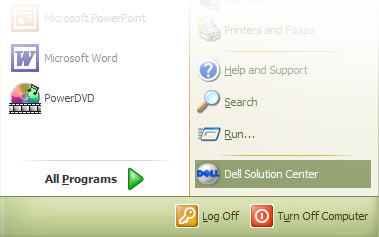
\includegraphics{images/startmenu}

3. Type cmd and press return

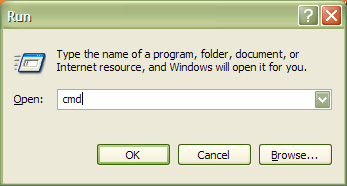
\includegraphics{images/cmd}

4. Type chuck and press return, you should see:

\chuckterm{
    \prompt chuck
    
    [chuck]: no input files... (try --help)
}

\section{Source Installation}

To build chuck from the source (Windows users: it's possible to build ChucK
from both Visual C++ 6.0 and from cygwin - this section describes the cygwin
build): 

1. Go to the src/ directory (replace chuck-x.x.x.x with the actual 
directory name):

\chuckterm{
   \prompt cd chuck-x.x.x.x/src/
}


2. If you type 'make' here, you should get the following message:

\chuckterm{
   \prompt make\\
   \chuckbuild: please use one of the following configurations:\\
       make osx, make osx-intel, make win32,\\
       make linux-oss, make linux-alsa, make linux-jack
}

Now, type the command corresponding to your platform... 

for example, for MacOS X (power-pc):

\chuckterm{\prompt make osx}

for example, for MacOS X (intel):

\chuckterm{\prompt make osx-intel}

for example, for Windows (under cygwin):

\chuckterm{\prompt make win32}

3. If you would like to install chuck (cp into /usr/bin by default). If you 
don't like the destination, edit the makefile under `install', or 
skip this step altogether. (we recommend putting it somewhere in your 
path, it makes on-the-fly programming easier)

\chuckterm{
   \# (optional: edit the makefile first)\\
   \prompt make install
}

You may need to have administrator privileges in order to install ChucK. If you 
have admin access then you can use the sudo command to install.

\chuckterm{
   \prompt sudo make install
}

4. If you haven't gotten any egregious error messages up to this point, 
then you should be done! There should be a `chuck' executable in the 
current directory. For a quick sanity check, execute the following (use 
`./chuck' if chuck is not in your path), and see if you get the same output:

\chuckterm{
   \prompt chuck
   [chuck]: no input files...
}

(if you do get error messages during compilation, or you run into some 
other problem - please let us know and we will do our best to provide 
support) 

\rule{1in}{.5pt}

You are ready to ChucK. If this is your first time programming in 
ChucK, you may want to look at the documentation, or take the ChucK 
Tutorial ( \href{http://chuck.cs.princeton.edu/doc}{http://chuck.cs.princeton.edu/doc/}). 

ThanK you very much. Go forth and ChucK - email us for support or to make a 
suggestion or to call us idiots.

Ge + Perry
